\newpage
\section{Genomic combination}

\subsection{Sanger assembly: overlap-layout-consensus algorithm}

We can think about the reads as the potential vertexes that we 
want to connect with edges. 
So \textbf{we want to find the edges connecting our reads}.

The sequence-overlaps between reads will allow us to define the 
edges of our \textbf{Hamiltonian path}.
  
So it is possible to build the path with simple greedy algorithms
without the need to calculate all the possible hamiltonian paths to 
find the best fit.

If we have n reads, we will need to calculate $n^2$ possible overlaps.\\

With the sanger assembly we have to:
\begin{enumerate}
  \item calculate pairwise alignments of all fragments
  \item choose two fragments with the largest overlap
  \item merge chosen fragments
  \item repeat setp 2 and 3 until only one fragment is left
\end{enumerate}

The problem with this approach is that it takes a lot of time (the complexity
is exponential). How can we solve this problem?\\

\subsection{Shotgun fragmentation and assembly}

Consider this minute single stranded DNA circular genome, 14 bases long.
Random fragments can start from any of the 14 positions.
We can imagine to produce reads of just 3 bases, considering that the
reads included in repeats will be found at a higher rate.

\begin{figure}[H]
  \centering
  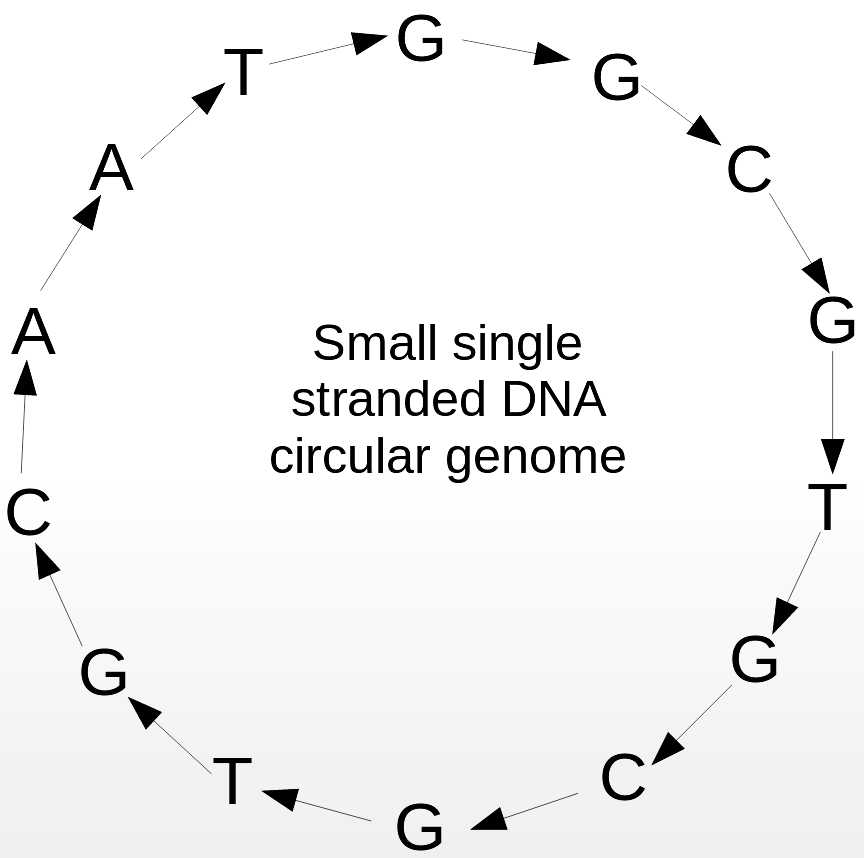
\includegraphics[scale=0.25]{smalldna}
  \caption{example DNA, can you imagine? :)}
  \label{fig:smalldna}
\end{figure}

The reads are:

\texttt{GGC, GCG, CGT, GTG, TGC, GCG, CGT, GTG, TGC, GCA, CAA, AAT, ATG, TGG}

Classic methods for de novo assembly are based on connecting reads by overlaps.\\
 
\textbf{reads $=$ graph nodes}
 
\textbf{overlaps $=$ edges}\\

Since there may be repeats, the graph may not be linear. 
The assembly algorithm must find the most plausible path in the graph.

\begin{figure}[H]
  \centering
  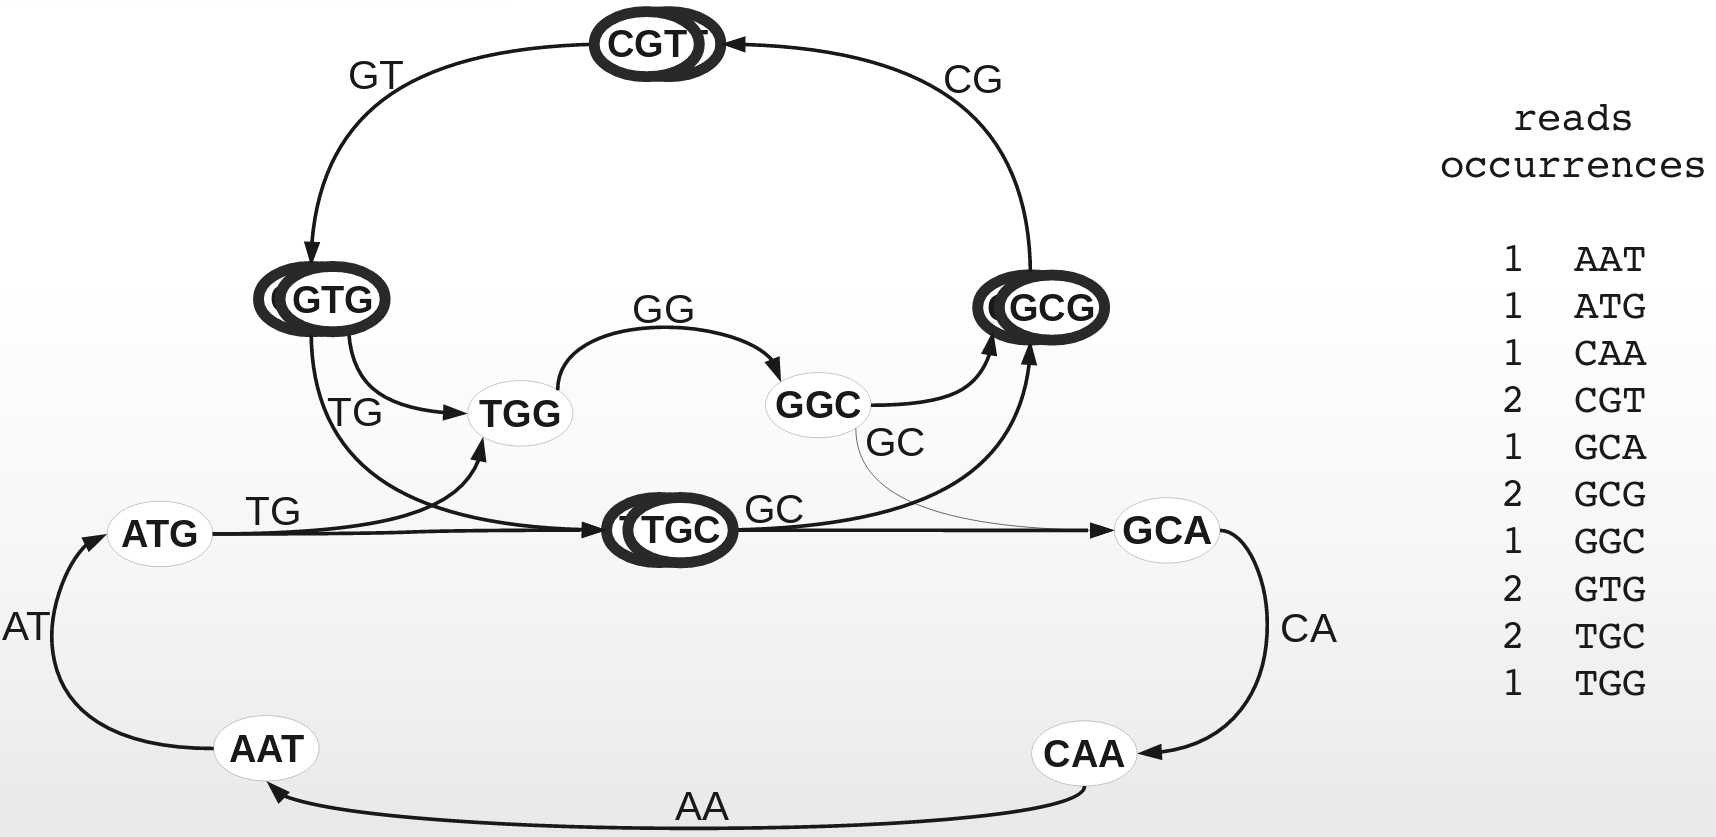
\includegraphics[scale=0.25]{graphreads}
  \caption{graph with reads and occurences}
  \label{fig:graphreads}
\end{figure}

In our graph (figure \ref{fig:graphreads}) we should find a path 
going over each node \textbf{only once}.

Some sequences occurring at a higher rate may be repeated more 
than once (bold circles) and we could represent them by two or more nodes
with the same sequence. 

Finding a path in a graph, passing \textbf{once over each node}, is known as
\textbf{Hamiltonian path problem}.

A Hamiltonian \textbf{cycle} is a Hamiltonian path that starts and ends at
the same point.

This lead to the \textit{Hamiltonian Problem}, that is a
very difficult problem (NP-hard). \\

Another solution is to implement an \textbf{Eulerian path}, that goes
\textbf{once over each edge}, and it's a simpler problem.

In the specific case of sequence assembly, an  Eulerian path can be
obtained by considering the reads as edges and the overlaps as vertices.\\

\textbf{reads $=$ edges}
 
\textbf{overlaps $=$ graph nodes}\\

\begin{figure}[H]
  \centering
  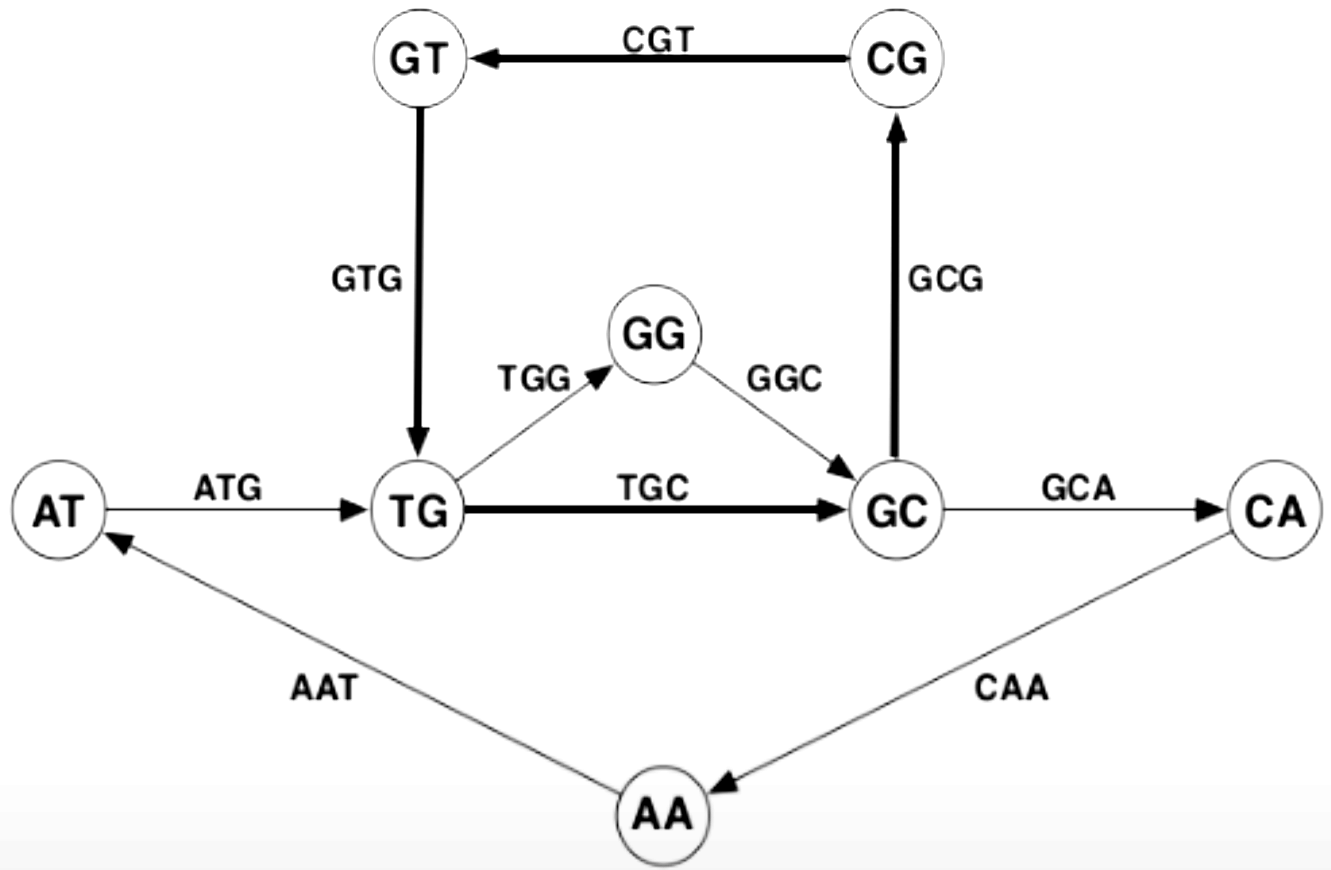
\includegraphics[scale=0.25]{eulerianreads}
  \caption{graph with reads as edges}
  \label{fig:eulerianreads}
\end{figure}

Also in this case we want to walk once over each read, but 
now the reads are edges instead than vertices.

\paragraph*{Euler's Theorem} A graph has a Eulerian \textbf{cycle} if the
degree of every vertex is \textbf{even} (pari).

If the graph has directions (one way streets), then a Eulerian
cycle exists if each vertex has the same number of entering and exiting edges. \\

\textbf{Computationally the two problems are very different}.

The Eulerian solution doesn't solve the problem of overlaps.\\

Two important points:

\begin{itemize}
	\item We are dealing with NGS reads. They could be billions and we cannot
search for the overlaps of all reads against all, that has a complexity
$n^2$. Ideally we would like to have a complexity proportional to the number
of reads.
	\item NGS reads may have different lengths. Which length should be
consider for the reads (represented by the edges of the graph) and
which length should we consider for the overlaps (represented by the vertices)?
\end{itemize}

Ideally, the longer reads and overlaps are and the better it should be.
However, reads may contain sequencing errors.

Consider a read of 80 bases with an error. 

The wrong read will generate a false edge: not only any useful information
contained in that read is lost, but a wrong edge is generated, producing noise.

Instead, if we split the read into 3 words of 25 bases we would get 2
perfectly right words and one wrong.

\subsubsection{Be Bruijn graphs and Eulerian path}

Consider the following statements:

\begin{enumerate}
	\item Given an alphabet of $n$ characters, there exist $n$ words of
length $l$ whose suffix is $w$ (each such word is obtained by adding one of
$n$ letters to the beginning of $w$)
	\item The indegree of each vertex in $B(n,l)$ is also $n$
	\item Every vertex of $B(n,l)$ has indegree and outdegree both equal to $n$
	\item Euler's Theorem implies that $B(n,l)$ must have an Eulerian cycle
\end{enumerate}

For DNA sequences, we can consider that given a kmer of length k,
existing within a DNA sequence, the next kmer shifted by one position will be
one of the possible 4 words obtained by removing one character at one end of
the previous word and adding one of the 4 possible characters to the other end.

\begin{figure}[H]
  \centering
  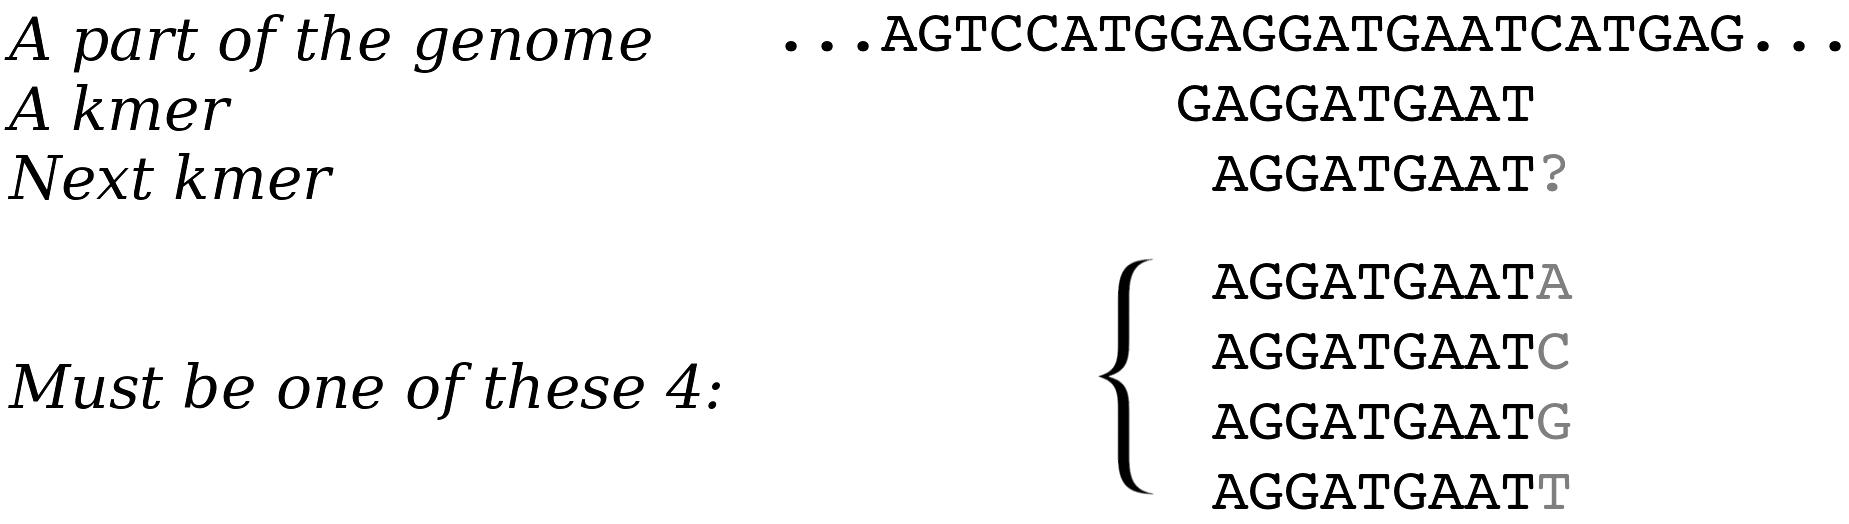
\includegraphics[scale=0.2]{nextkmer}
  \caption{next kmer}
  \label{fig:nextkmer}
\end{figure}

This observation allows to build graphs very easily and make possible to search
for Eulerian paths, thus assembling the kmers into contigs.

If we knew all the kmers present in the genome, then we would be able to find
the right next kmer.

This is possible only if the kmer is present only once in the genome;
therefore kmers must be long enough, otherwise the overlap (?) would occur by
chance, and shouldn’t be repeats.

This is the best solution for now, and uses a study published by the
matematician Be Bruijn.
Steps for the solution:
\begin{enumerate}
  \item In pratical terms, a shotgun library is made and it is sequenced at a
reasonably high coverage, for instance 60x

\begin{figure}[H]
  \centering
  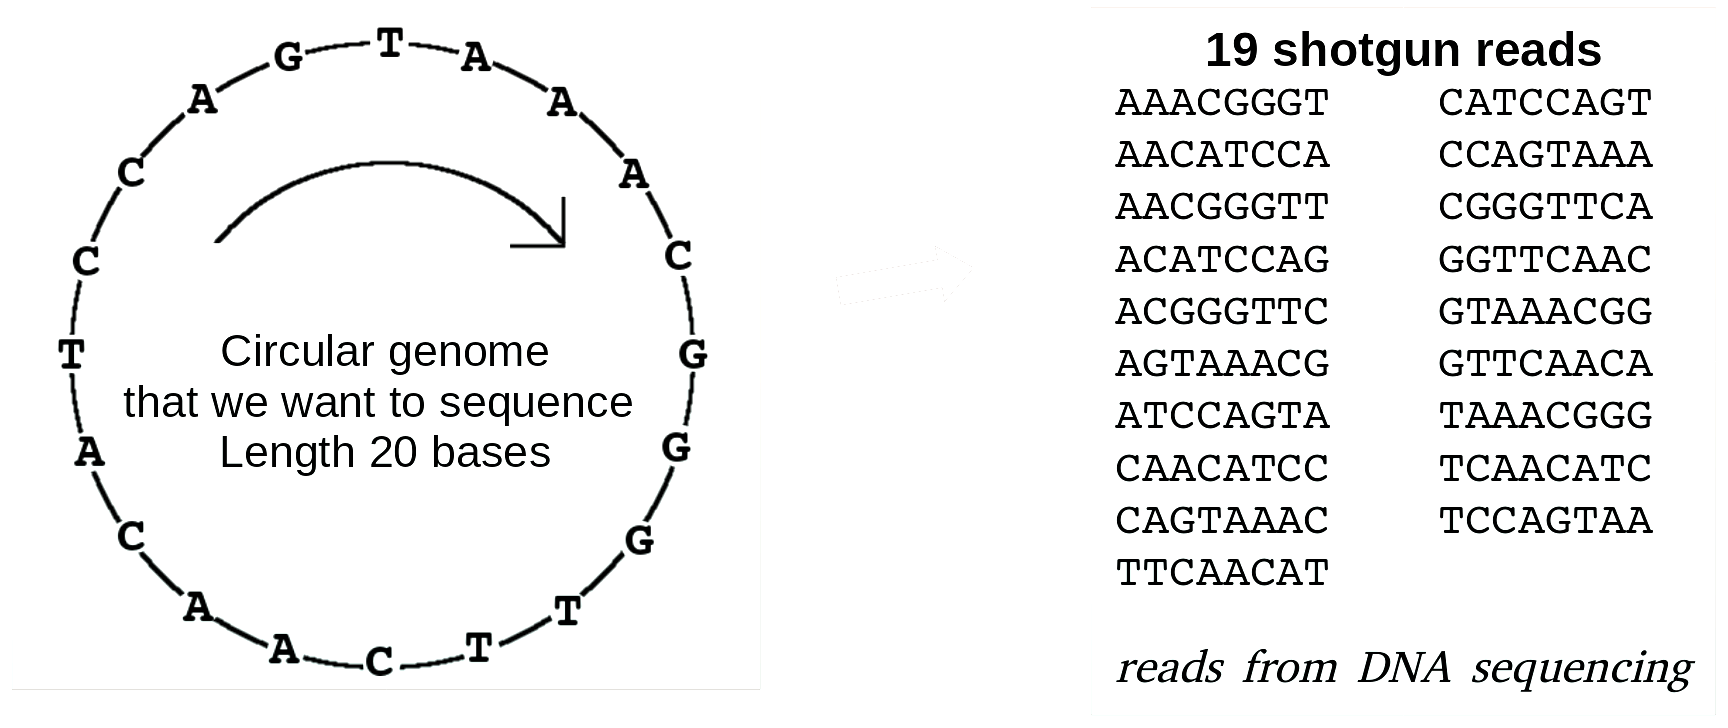
\includegraphics[scale=0.2]{dnareads2}
  \caption{dna sequence and reads}
  \label{fig:dnareads}
\end{figure}

  \item The resulting fastq file is read once, and all the kmers are counted.
This process will produce a list of all the kmers and their frequency
(in the example \textbf{k = 3})

\begin{figure}[H]
  \centering
  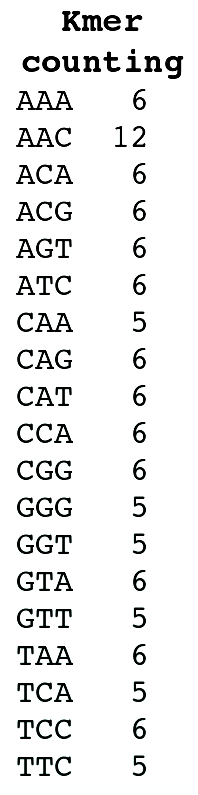
\includegraphics[scale=0.3]{kmer_counting}
  \caption{kmer frequency}
  \label{fig:kmer_counting}
\end{figure}

  \item We can start from any kmer that was found at the expected frequency and
we can extend the resulting conting by moving one position at a time. At every
step we will need to choose one of the 4 possible kmers. This will be done by
looking at the list of kmers. If there are no repeats then only one of the four
kmers should be present in the list.
(in the example there are repeats).

\begin{figure}[H]
  \centering
  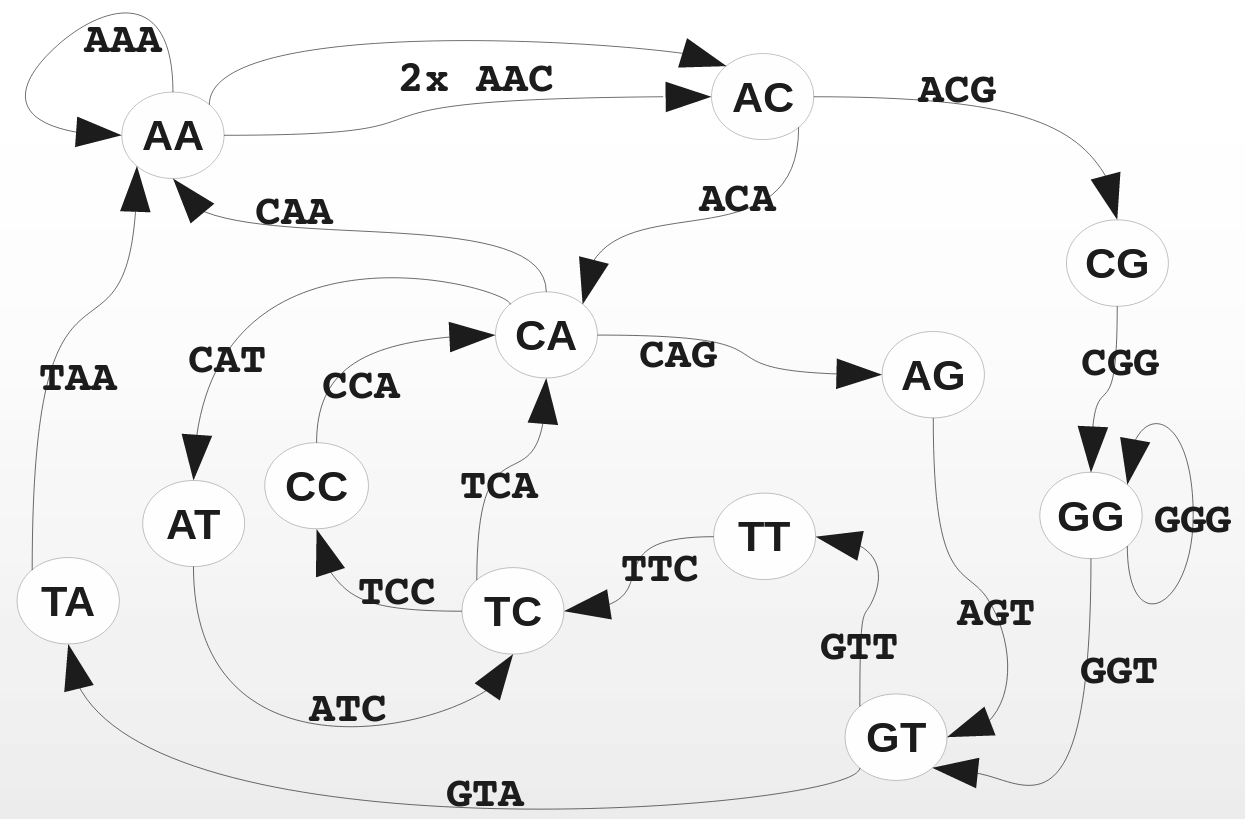
\includegraphics[scale=0.2]{graph2}
  \caption{graph produced. We want to find an \textbf{eulerian path}}
  \label{fig:graph2}
\end{figure}

\end{enumerate}

The method shown is computationally simple.
You need to read the reads only once to produce the table with all the kmer
counts.

Then you can start from any kmer (edge), placing the suffix as a node to
move forward and the prefix as a node to move backward.
Then you can continue the path by finding existing  edges (kmers)
compatible with the new nodes.

This is done by looking at the table with the kmer counts.
Valid paths should go through kmers with some counts.

Kmers with very few counts could be generated by errors, producing kmers
similar to existing ones.

Instead, kmers with more counts than expected could be generated by
repeats, like AAC in the example that is found with double frequency than
expected and indeed is a repeated sequence.

This should be represented by two edges, meaning that the path should go over
AAC twice.

In the example there are too many nodes with multiple edges.

Therefore there are several possible solutions.
We know that we can resolve the cycle because all the nodes have the 
same number of entries and exits, but we cannot say which is the correct one.

\begin{figure}[H]
  \centering
  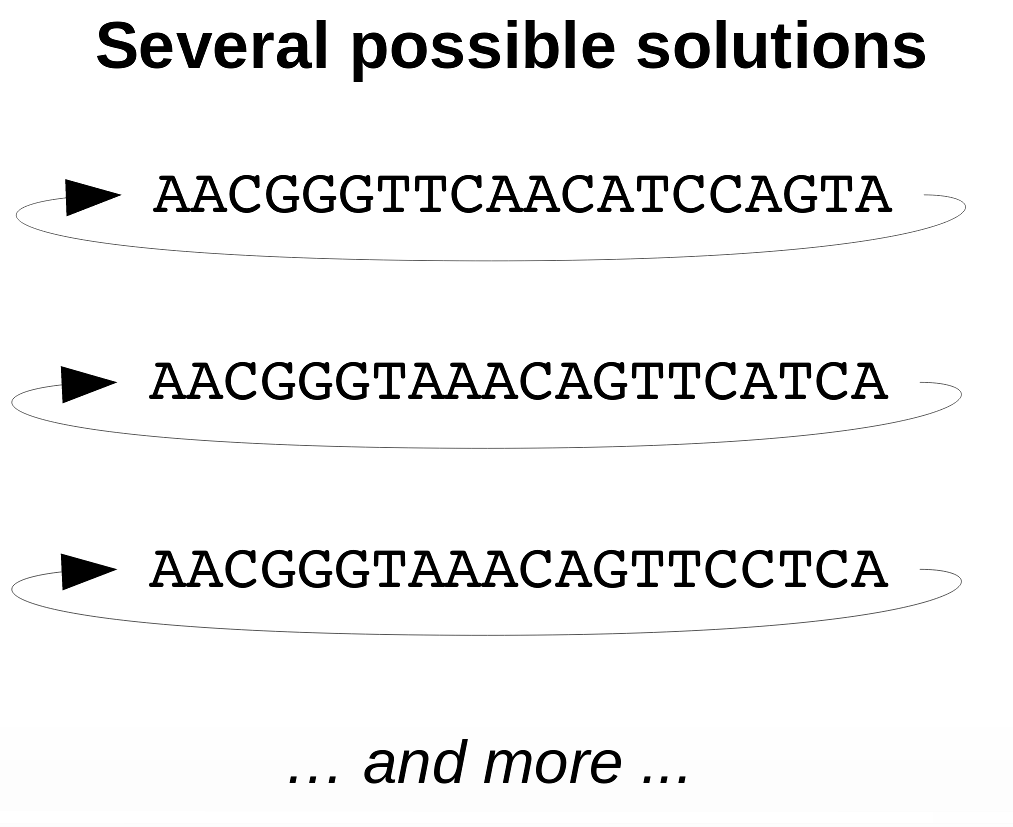
\includegraphics[scale=0.2]{possible_solutions}
  \caption{possible eulerian paths for the example}
  \label{fig:possible_solutions}
\end{figure}

\subsection{Another example}

In next example the same set of reads is used, but the length of kmer is
\textbf{k = 4}. See figure \ref{fig:example2}.

With k=4 now we have only one node (AAC) with double branches, 
thus we can read two relatively long linear “contigs”: 
\texttt{AACATCCAGTAAAC} and \texttt{AACGGGTTCAAC}, both longer than the
original reads. 

\begin{figure}[H]
  \centering
  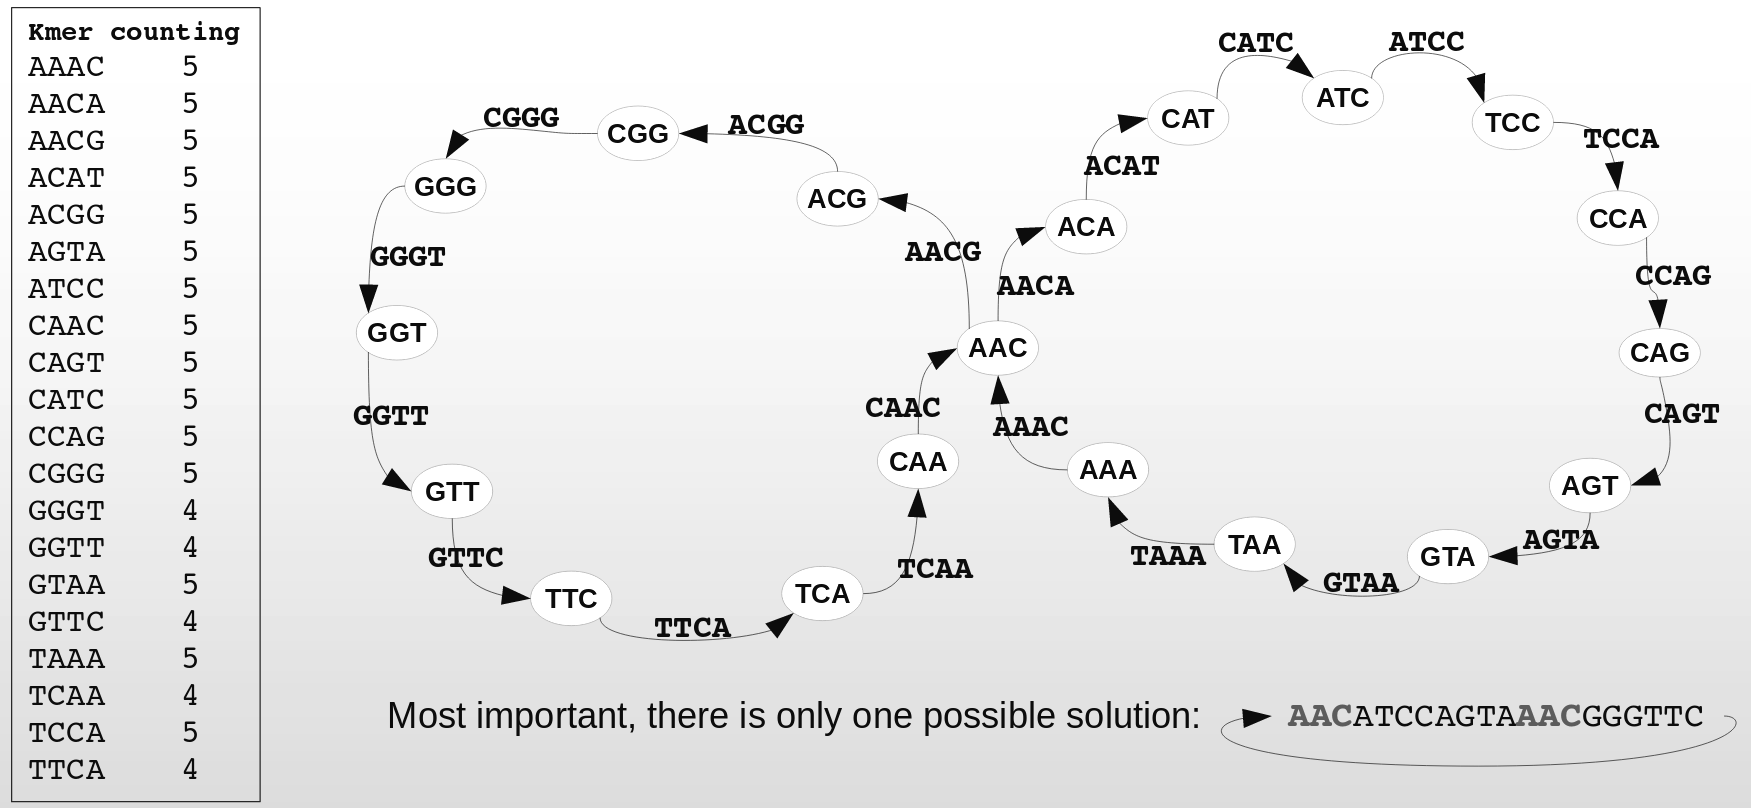
\includegraphics[scale=0.25]{example2}
  \caption{another example}
  \label{fig:example2}
\end{figure}

... and there is only one possible eulerian path.

\paragraph*{De Bruijn graphs and mate pairs}

\begin{itemize}
	\item Things are a little more complicated. With DNA sequences we need to
consider that the same fragment of double stranded DNA could be sequenced
from 2 different ends.

For instance ACCTG and CAGGT should be counted as if they were the same
sequence. 
	\item What is the best kmer length? It should be the longest possible, but
it is not so because reads may contain errors.
One sequencing error in the middle of a read will produce k wrong kmers.
With our current technology we obtain the best results with k values around
20-30 bases.
	\item Genomic sequences are full of repeats and usually the De Bruijn
graphs have many many branches with the consequent problem of a vast number
of possible solutions.
	\item To help in the identification of the right path (i.e. the right
assembly) we can use Mate Pair libraries.
Several programs that take advantage of DeBruijn graphs together 
with mate pairs have been implemented, for instance Velvet. 
\end{itemize}
